% $Id: nsf_description.tex 3089 2012-10-23 21:38:10Z nkraft $


\part{Computing Research Infrastructure Concept}
A \textit{Systematic Literature Review (SLR)} is a rigorous, standardized process by which researchers identify and analyze published evidence to draw broad conclusions about a phenomenon or research question.
The systematic, comprehensive, and reproducible nature of SLRs leads to findings that are less prone to bias and omissions than are s typical of the traditional \textit{ad hoc} literature review.
Given the frequency of empirical studies in software engineering (SE), the domain is well-suited for SLRs.
Although SLRs are increasingly recognized as vital to the SE discipline, the lack of infrastructure to support this effort-intensive, largely manual process results in barriers that inhibit their widespread adoption.
Building upon the results of our CI-P grant (NSF-1305395), the primary goal of this CI-NEW project is to build infrastructure to reduce these barriers and increase adoption of SLRs in SE.
For the sake of this proposal, we define \textit{infrastructure} to include both the back-end data storage and interchange, as well as the front-end user tools that support specific SLR steps.
Our target community comprises SE researchers who already conduct SLRs, SE researchers who will be more likely to conduct SLRs if the barriers are removed, SLR tool builders, and industry consumers of SE research results. 
The primary objectives of this CI-NEW project are to: 
\begin{itemize*}
	\vspace{-6pt}
	\item Build an extensive SLR support infrastructure;
	\item Ensure the infrastructure is flexible enough to incorporate existing and new tools; and
	\item Validate the usefulness of the infrastructure with members of the target community.
\end{itemize*}
\vspace*{-4pt }


\section{Introduction}
\label{sec:intro}
% $Id: sec_intro.tex 3089 2012-10-23 21:38:10Z nkraft $

The review of existing literature is the foundation of all new research. In SE, these reviews have traditionally been performed in an \emph{ad hoc} manner. To provide some structure to the literature review process, medical researchers defined the SLR process. While SLRs have been commonplace in medicine, they are a recent phenomenon in SE largely due to significant barriers that inhibit their wider adoption, e.g., the process is labor intensive and tool support is lacking. The goal of the proposed infrastructure is to lower the barrier for researchers who want to perform SLRs. The proposed infrastructure will also provide researchers with a platform for community interaction and data dissemination. We expect that the infrastructure will increase not only the quantity, but also, more importantly, the quality of SLRs and SE research in general. %We also expect the proposed infrastructure to foster industry adoption. [[Do we need last sentence??]]

The initial step of a new research endeavor is a review of previous work to properly ground the new research. The most common method of examining previous work is via literature review. A literature review can also have other goals, such as, summarizing the current state of knowledge about an area as a service to the community. Regardless of the goal of the literature review, a researcher can perform the review in the traditional, unsystematic, fashion, that is, by conducting database searches and following references or the researcher can use a more systematic method. 

An SLR is a formal, repeatable method by which a researcher can identify, evaluate, and interpret the available research about a question or topic area. The primary difference between an SLR and and \emph{ad hoc} review is the level of advanced planning in an SLR. Prior to conducting the review, the researchers develop a protocol that documents: the research question(s) to guide the review, the search strategy (including specific databases and keywords), the criteria for choosing appropriate papers, a quality assessment method for the papers, the specific information to be extracted from each paper, and a plan for synthesizing the information from the set of papers to draw a conclusion. By using this systematic process, researchers are much less likely to accidentally omit important papers from the literature review.

Medical researchers, practitioners, and policy makers have long relied on SLRs, because they integrate up-to-date, reliable, and critical information that support important decisions. Seeking these same benefits, the SE community has recently begun publishing SLRs. Indeed, with the growing emphasis on empirical research in SE, SLRs are of critical importance because they allow researchers to bring together disparate evidence to understand the effects of various SE tools, techniques and methods. Unfortunately, though production and dissemination of SLRs is key to the maturation of SE and to the adoption of SE research practices by industry, conducting an SLR is a difficult and time-consuming process. Based on our own SLR experiences, a review of over 200 SLRs, and a survey of over 50 SLR authors, we have identified four key barriers to wider adoption. Section 2 discusses each of these barriers in more detail.

First, the process of systematically identifying relevant papers is largely manual and thus very labor intensive. This process is more difficult when research topics cross traditional disciplinary boundaries, as many interesting topics increasingly do. While some advancement has been made in database functionality, as a discipline, we still lack adequate tools to assist in the extraction and compilation of relevant information from existing research. Using most common search engines for SE literature (i.e., IEEExplore, ACM, or Google Scholar), a search may yield thousands of results, of which a large percentage may be irrelevant for various reasons (i.e., overloaded terminology or simply contain the right word combinations by chance). In addition, because databases are not mutually-exclusive, the result set will likely contain duplicates, which must be manually parsed by the researchers.

Second, there is little tool support for collaborative SLRs. After identifying the relevant set of articles, multiple researchers must extract important information from each paper and compare the results for consistency. Again, this step is typically performed manually. There is no tool support to ease this process and to aid in the inter-rater reliability assessment necessary to evaluate the accuracy of the extracted information.

Third, there is no mechanism to store the data extracted from papers so that it can be updated and reused. It is quite likely that the same paper may be relevant to multiple SLRs. While the data extracted from a paper may differ somewhat depending on the research questions, there will likely be a lot of common data items. Because there is no central repository for storage of extracted data, researchers must fully repeat this extraction process for each new SLR. Such a repository would not only reduce effort by enabling a researcher to extract only the additional data relevant to the new research question(s), but also facilitate collaboration by allowing researchers to identify others working on similar topics.

Finally, there is  no mechanism to enable SLRs to evolve over time. Ideally, an SLR should be a ``living'' document that could evolve as new research results become available. Because current publications are static, appropriate infrastructure is needed to support the evolution of SLR results by allowing researchers to easily create new versions or fork off related topics. Making SLRs living documents that incorporate the latest research results will allow them to be more useful both to researchers and practitioners.

To address these barriers and to provide a platform to encourage more researchers to conduct SLRs, there is a need for new infrastructure. The goal of this planning grant is to build upon our initial experiences to develop a complete picture of the community needs for this infrastructure. By interacting with the community SLR authors, we will clarify the set of problems for which infrastructure is particularly needed. In addition, we will also interact with the community to ensure that by the end of the planning grant we have a concrete proposal for the implementation of the infrastructure that the community will find useful and beneficial.

\paragraph{Intellectual Merit}

Literature reviews are an integral part of any new research activity. As such, it is critical that researchers are able to identify as complete a set of related literature as possible. This project will produce a plan to develop and deploy such infrastructure. Specifically, the resulting infrastructure will facilitate current and future research %in the following ways:
in that it will:
\vspace*{-4pt}
\begin{itemize*}
%\item It will enable researchers to more easily perform SLRs by reducing the manual effort required and improving the accuracy of the result
\item Enable researchers to perform SLRs more easily by reducing the manual effort required and by improving the accuracy of the result
%\item It will serve as a repository of all related literature about a research topic that can be kept current through addition of newly published articles
\item Serve as a repository of all related literature about a research topic that can be kept current through the addition of newly published articles
%\item It will aid additional research by providing a repository of peer-reviewed data extraction sheets to the research community for exploration and use in meta-analysis
\item Foster additional research by providing a repository of peer-reviewed data extraction sheets to the research community for exploration and use in meta-analysis
%\item It will serve as a community hub to facilitate geographically dispersed collaboration efforts and to enable social networking regarding the results of SLRs
\item Serve as a community hub to facilitate geographically distributed collaborations and to enable social networking regarding the results of SLRs
\end{itemize*}
\vspace*{-4pt}

\paragraph{Broader Impacts}

By lowering the barriers to performing SLRs and enabling more SLRs to be produced, the proposed infrastructure will: %have the following broader impacts:
\vspace*{-4pt}
\begin{itemize*}
\item Enable a larger portion of the SE community, especially new researchers, to conduct SLRs
\item Increase the prevalence of summarized results that can inform research and practice
\item Make the results of a review to be accessible to a larger audience

\end{itemize*}
\vspace*{-4pt}

In addition, because SLRs are often publishable in their own right, and because all PhD students must perform some type of literature review as part of their work, the proposed infrastructure will enable PhD students to obtain an additional publication in the course of their work.

The proposal is organized as follows. The remainder of Part I provides background on SLRs and existing tools. Part II describes our preliminary work to identify community needs with regards to infrastructure requirements (Section~\ref{sec:prelim:needs}) and proposed solutions (Section~\ref{sec:prelim:tools}). Part III details the work we plan to conduct as part of this planning project to validate the information in Part II. Part IV lays out the plan for completing the proposed work. Finally Part V describes the qualifications of the investigators.

% vim:syntax=tex


\section{Systematic Literature Review Process}
\label{sec:process}
% $Id: sec_process.tex 3089 2012-10-23 21:38:10Z nkraft $

Kitchenham ported the SLR process from the medical field to SE. The process, as prescribed by Kitchenham~\cite{Kitchenham:04,Kitchenham_Charters:07}, consists of three primary phases: review planning, review execution, and review documentation.

During the \textbf{planning phase}, the researcher defines a protocol that guides SLR execution. The goal of the protocol is to reduce researcher bias and provide a repeatable, transparent process for conducting the SLR. The protocol should contain, at a minimum, the following information:
\begin{enumerate*}
	\item[P1.]{Motivation for conducting the SLR}
	\item[P2.]{Research question(s)}
	\item[P3.]{Search strategy - including databases to be searched and search string(s)}
	\item[P4.]{Strategy for identifying primary studies (i.e. inclusion and exclusion criteria)}
	\item[P5.]{Quality assessment criteria}
	\item[P6.]{Data extraction form}
\end{enumerate*}
\vspace*{-8pt}

An independent expert or panel reviews the protocol for completeness and validity. If at any point during the SLR execution the researchers must change the protocol, the expert or panel should re-review the revised protocol.

During the \textbf{execution phase}, researchers proceed through five steps:
\begin{enumerate*}
	\item[E1.]{Identify relevant research by executing the defined search strategy}
	\item[E2.]{Select primary studies by applying the inclusion and exclusion criteria}
	\item[E3.]{Assess study quality using the quality assessment criteria}
	\item[E4.]{Extract required data into data extraction forms}
	\item[E5.]{Synthesize data to draw conclusions}
\end{enumerate*}
\vspace*{-8pt}

Researchers apply the search terms to multiple databases. Then the researcher(s) use the inclusion and exclusion criteria to reduce the results of the search process, using titles first, then abstracts, then full text. During each iteration, the researcher(s) eliminate prospective studies only when it is clear that the study is not relevant. After selecting the primary studies, the researchers perform a quality assessment of each selected study. The studies are then weighted based upon the results of the quality assessment. Finally, the researchers extract important data from all included studies. The resulting data set then forms the basis for the data synthesis. To reduce researcher bias in the process, members of the research team perform each step independently and then meet to review the results and resolve any conflicts. 

Lastly, during the \textbf{documentation phase} the researchers use all of the information described in the protocol, along with the results of the execution of the protocol to document the review in some type of publication. This phase consists of the following steps:
\vspace*{-4pt}
\begin{enumerate*}
	\item[D1.]{Specify dissemination strategy}
	\item[D2.]{Format SLR report}
\end{enumerate*}
\vspace*{-4pt}

\subsection{Existing tools}
\label{sub:existing:tools}
The SLR process originated with the The Cochrane Collaboration, the primary organization that organizes and disseminates SLRs in medicine. With the long history of SLRs, we expected to find some sophisticated suport tools. We did locate one toolset, the RevMan/Archie combination utilized by the Cochrane Collaboration~\cite{RevMan:11}. RevMan focuses primary on the documentation phase of SLRs performed under the guidelines of the Cochrane Collaboration.  RevMan includes facilities for the preparation of formatted tables used in the reviews and for tracking the revisions of a review over time.  Archie is the central repository, or backend for the RevMan application and is used to store completed reviews. Neither tool appears to provide much functionality to support the planning or execution phases of the SLR process.

With the increasing prevalence of SLRs in SE, we were surprised to find only two tools that support the SLR process within SE. First, StArt~\cite{Fabbri_et_al_2012} is a desktop based application design to assist an individual researcher in designing and conducting an SLR that follows the process originally described by Kitchenham~\cite{Kitchenham:04}. To use StArt, a researcher inputs protocol elements, including: research questions, databases, and study selection criteria. These elements then become attributes of the steps in the execution phase of the SLR. StArt also provides some assistance for ``snowballing,'' the process in which researchers trace the citations of a paper forward and backwards, by comparing identified studies with the references of the studies. StArt also includes visualizations that assist in the development of the search strings and the documentation of the review.

Second, SLuRp~\cite{Bowes_et_al_2012} is a web based tool that functions as the central repository for an SLR research team. The repository provides a common storage location for the SLR protocol, PDF copies of the studies under review, and associated reference information. Additionally, SLuRp provides facilities to manage the assignment of studies for review to the different researchers on the team and to collect the results of these reviews.

% vim:syntax=tex



\part{Preliminary Work}
% $Id: part_prelim.tex 3073 2012-10-23 17:55:38Z jcarver $

We have performed initial work to gather community needs and identify necessary characteristics and features for the infrastructure. Section~\ref{sec:prelim:needs} describes the community needs we have identified through our own experiences and our interactions with the community. Section~\ref{sec:prelim:tools} describes our current view of the infrastructure required to address the identified community needs.

% vim:syntax=tex


%\section{Proposed Requirements}
\section{Identification of Community Needs}
\label{sec:prelim:needs}
% $Id: sec_prelim_needs.tex 3089 2012-10-23 21:38:10Z nkraft $

As a starting point for planning the infrastructure, we have identified a set of important community needs, which will be iterated upon during the course of the project. The important community needs we identified include, improved support for:
\vspace*{-4pt}
\begin{enumerate*}
	\item{Coordination among multiple (possibly distributed) researchers}
	\item{Protocol review by the community}
	\item{Interaction with different literature databases}
	\begin{enumerate*}
		\item{Federated search}
		\item{Search string manipulation and translation}
		\item{Duplicate result elimination}
		\item{External citation management tool interoperation}
	\end{enumerate*}
	\item{Quality assessment}
	\item{Data extraction}
\end{enumerate*}
\vspace*{-4pt}

Section~\ref{sub:sources} describes the three data sources used to gather these needs. Section~\ref{sub:analysis} provides a detailed analysis of the data sources to illustrate the origing of these community needs.

\subsection{Overview of Data Sources}
\label{sub:sources}

To gather community needs, we used three data sources: a graduate course by PI Carver (Section~\ref{sub:SLR:course}), a review of published SLRs (Section~\ref{sub:SLR:review}), and a survey of SLR authors (Section~\ref{sub:SLR:survey}).

\subsubsection{PI Carver's SLR Course}
\label{sub:SLR:course}

In Spring 2012, PI Carver taught a graduate ``Advanced Empirical Software Engineering'' course. There were eight PhD students enrolled in the course (four Computer Science PhD students and four Management Information Systems PhD students). The main focus of this course was for the students to learn about and conduct SLRs. As such, the course had two primary goals:
\vspace*{-4pt}
\begin{enumerate*}
	\item Each student conducted an SLR as a semester-long  project. Realizing that most SLRs cannot be completed within one semester, it was expected that work would continue beyond the semester to make these SLRs publishable. At this point, two of these papers have been accepted in conferences~\cite{Thompson_et_al_2012,Kakar_Carver_2012}, at least five other papers will be submitted to various journals in the near future, including \emph{European Journal of Information Systems} and \emph{Information and Software Technology}, and most of them will become part of the students' dissertations.
	\item Second, throughout the semester, class time was devoted to discussing each student's SLR and to evaluating the SLR process. Each student wrote a report at the end of the semester describing their SLR process, noting where they had difficulties, and suggesting improvements to the SLR process.
\end{enumerate*}
\vspace*{-4pt}

In addition, each student acted as a second reader for the SLR of one of their classmates. PI Carver oversaw all SLRs, provided input on the protocols and helped to resolve any conflicts during the paper selection/data extraction process. Due to the effort required to conduct these reviews, it was not possible for every paper to be reviewed by two reviewers. So, at each elimination stage of the SLR process (i.e. title elimination, abstract elimination and full paper elimination), the second reader reviewed a random subset of 10-20\% of the excluded papers to ensure that the primary author was not prematurely excluding papers that could be relevant. When the primary author reached the data extraction stage, the second reader reviewed the full data extraction for a subset of the papers.

In addition to the interaction among the primary author and the second reader throughout the semester, a large portion of the class meeting time was devoted to discussing each SLR. Each student had the opportunity to present his protocol and received feedback from his classmates. The class also spent a substantial amount of time discussing the logistics of the SLR process and identifying common problems encountered by multiple students. By the end of the course each student produced two deliverables:
\vspace*{-4pt}
\begin{enumerate*}
\item An initial version of the SLR, which in most cases needed further revision to become publication-ready; and
\item A report describing his experiences with following the standard SLR process, including specific areas in which he encountered difficulties. It is these reports that provided the bulk of the information described Section~\ref{sub:analysis}.
\end{enumerate*}
\vspace*{-4pt}

\subsubsection{SLR Literature Review}
\label{sub:SLR:review}

For the second source of data, we performed a thorough literature search and identified 214 published SLRs. We analyzed those SLR papers to identify strengths and weaknesses in the current SLR process, including areas in which tool support could be helpful. During the review of these papers, we used the following data extraction process:
\vspace*{-4pt}
\begin{enumerate*}
\item Determine whether the SLR protocol was explicitly described
\item Review the description of the protocol to:
\vspace*{-4pt}
   \begin{enumerate*}
	\item Note databases used and the search strategy for those databases
	\item Note any deviations from Kitchenham's process (whether stated explicitly or not)
	\item Note any tools used
	\item Note any difficulties described about the process
   \end{enumerate*}
\vspace*{-4pt}
\item Look for a ``lessons learned'' section to get more details
\item Note anything else particularly interesting about the SLR process in the paper
\end{enumerate*}
\vspace*{-4pt}
The information extracted from this analysis is included in Section~\ref{sub:analysis},
and the list of 214 published SLRs is included among the cited references at the end of this proposal.

\subsubsection{Survey of SLR Authors}
\label{sub:SLR:survey}

Finally, to obtain more detailed insight into the SLR process, we developed a list of SLR authors from the list of published SLRs identified in Section~\ref{sub:SLR:review}. We sent a survey to all of those authors that asked them to detail: the SLR process followed, where they had difficulties in the SLR process, where they spent their time during the SLR process, and which aspects of the SLR process were most in need of tool support. The results of the 50+ survey responses are included in the discussion in Section~\ref{sub:analysis}.

\subsection{Analysis of SLR Process}
\label{sub:analysis}

This section uses data gathered from the three data sources described in Section~\ref{sub:sources} to analyze the steps in the SLR process. The goal of the analysis is to identify aspects of the SLR process that SLR authors found particularly difficult, highlighting community needs for tool support of the SLR process. This section is organized around the major phases of the SLR process: Section~\ref{sub:proto:plan} discusses general issues regarding Protocol Planning and Section~\ref{sub:proto:items} focuses on specific protocol items. For the sake of continuity, we discuss data from all three data sources together under each heading. As we discuss each phase of the SLR process, we specify the identified community needs.


\subsubsection{Protocol Planning}
\label{sub:proto:plan}

This section describes general information pertaining to protocol development. Information about detailed protocol items appears in Section~\ref{sub:proto:items}. During PI Carver's course, the students' stated that the frequent discussion of their protocols with each other and with PI Carver helped in the development and refinement of the protocols. The students also found it helpful for their SLR process to be guided by PI Carver, who is experienced in conducting SLRs. These experiences are not unique to PI Carver's course. Our review of the SLR literature suggests that many SLRs are performed by students as part of their thesis work. Guidance from a more experienced researcher/reviewer is crucial to the accuracy and success of the review~\cite{EMendes_2005}. The community needs identified in this phase are:
\vspace*{-4pt}
\begin{itemize*}
\begin{bfseries}
\item Protocols may have to be revised and edited during the SLR process
\item Protocols need to be socialized among peers for review and feedback
\item Novice researchers need the ability to interact with a more experienced research during the planning and execution of the SLR
\end{bfseries}
\end{itemize*}
\vspace*{-4pt}

\subsubsection{Protocol Items}
\label{sub:proto:items}

This subsection describes the results obtained for protocol items P2-P6.

\paragraph{P2. Research Questions}

The research question(s) are arguably the most important aspect of the protocol because they drive the remainder of the protocol. Based on the experiences in PI Carver's course, it is clear that the research question(s) have to be appropriately scoped. If they are too broad, they will generate too many papers to reasonably evaluate in one SLR. Conversely, if they are too narrow, they will not generate enough papers to draw useful conclusions. Scoping of the research question(s) is an activity in which feedback from more experienced researchers could be quite beneficial. The community need identified in this section is:
\vspace*{-4pt}
\begin{itemize*}
\begin{bfseries}
\item Research question(s) must be properly scoped
\item Expert feedback is beneficial to formulating appropriate research question(s)
\end{bfseries}
\end{itemize*}
\vspace*{-4pt}

\paragraph{P3. Search Strategy}

The search strategy includes database selection and creation of one or more search string(s) from the research question(s). Creating the search string(s) can be an iterative process as the researcher attempts to define the appropriate set of keywords and synonyms that cover the research space. This section first discusses issues with the databases and then issues with the search strings.

Regarding databases, SLR researchers typically search multiple databases, which may have different functionality. Based on the experiences in PI Carver's course, we can make the following observations regarding the databases. First, databases have different behavior regarding the search strings. For example, in some cases changing the order of the keywords changes the result set. In other cases, Boolean logic does not work as expected. As a result, researchers must develop a different set of search strings for each database. Second, the advanced search functionality differs across databases. In some cases, the advanced search interface returns different results than the basic search interface, even if the same search string is used. Third, there is a large overlap in the literature covered by the databases commonly used for SLRs, creating the need to identify and remove duplicate studies from the result set. Fourth, databases differ in the content and format of the citation information provided. Finally, the databases are not consistent in their behavior regarding bulk export of references to a citation manager.

Similar problems with the peculiarities of the databases were also reported by the papers in our literature review (e.g., \cite{LChen_et_al_2009,EladioDomınguez_et_al_2012,MuhammadSarmadAli_et_al_2010,LianpingChen_et_al_2011,SoniaMontagud_et_al_2012,MehwishRiaz_et_al_2009,IvoneiFreitasdaSilva_et_al_2011,EMendes_2005}). A relatively small number of researchers used EndNote to facilitate the removal of duplicate papers (e.g., \cite{LianpingChen_et_al_2011}) while most performed the task manually.

Regarding the search strings in general (i.e. not including differences among databases), the experiences in PI Carver's course resulted in the following observations. First, adding a '*' at the end of a key term helps to identify variant spellings. Second, when using a common term like ``Open Source,'' restrict the search to the title, abstract and keywords to limit the number of irrelevant hits. Third, in some cases a large number of relevant papers were not returned by the initial search, causing the search string to be refined based upon the results of a secondary search, i.e. reviewing references in the identified papers.

This information suggests the following community needs:
\vspace*{-4pt}

\begin{itemize*}
\begin{bfseries}
\item The ability to search multiple databases in one tool
\item Automatic (or semi-automatic) manipulation of search string to accommodate peculiarities of various databases
\item Automatic elimination of duplicate results
\item The ability to export all citations in a common format (i.e. BibTex or EndNote)
\end{bfseries}
\end{itemize*}
\vspace*{-4pt}

\paragraph{P4. Identification of Primary Studies}

Once the search results are identified, the next step is to determine which papers should be included in the SLR. There are two aspects to this process: the definition of the inclusion/exclusion criteria and the process of actually determining which papers belong in the review. The SLR author survey indicated that selecting appropriate papers was the third most difficult and second most time consuming aspect of the SLR process. It was also the aspect second most in need of tool support.

PI Carver's course resulted in the following observations about the inclusion/exclusion criteria: 1) there is a need to ensure that it conforms to the goals of the current review rather than just being reused from other SLRs; 2) there is a need for expert review; 3) it should be as specific as possible; and 4) it may have to be reviewed and edited during the search process. 

PI Carver's course also resulted in the following observations about the paper selection process: 1) review of the titles and abstracts may not be sufficient for eliminating papers; 2) there is a need for a citation manager to keep track of the references; 3) have to manually examine or write a script to handle duplicate results across databases; 4) when searching for specific terms or content that may not be evident in the title/abstract/keywords, the addition of a quick scan of the full text of the paper may be useful for quickly eliminating irrelevant papers; 5) this step was very time consuming, especially having multiple reviews of papers; and 6) it is difficult to coordinate meeting times. 

The literature review showed that other authors reported the same or similar problems. For example, some researchers noted the difficulty of duplicate removal~\cite{DIKSjoeberg_et_al_2005}. Researchers used various tools for managing the papers: a ``citation manager,''~\cite{MuhammadSarmadAli_et_al_2010} or EndNote~\cite{SusanMMitchell_et_al_2009,LianpingChen_et_al_2011,HongyuPeiBreivold_et_al_2010}.

\vspace*{-4pt}
This information suggests the following community needs:
\begin{itemize*}
\begin{bfseries}
\item There is a need for expert review of inclusion/exclusion criteria
\item The citations need to be managed within the tool
\item The tool needs to interoperate with external citation management tools (e.g., BibTeX, EndNote)
\item There is a need to automate the elimination of duplicate papers
\item There is a need for management of the review process among the SLR team
\end{bfseries}
\end{itemize*}
\vspace*{-4pt}


\paragraph{P5. Quality Assessment}

Once a set of candidate primary studies has been identified, the next step is to perform a quality assessment to determine whether any should be excluded due to the unreliability of their results. The results of the SLR author survey showed that quality assessment was the second most difficult and third most time consuming aspect of the SLR process.

The experiences from PI Carver's course resulted in the following observations. First, the quality assessment checklist should be part of the data extraction form. Second, the quality criteria must be relevant to the specific topic and not just reused from a prior SLR. Third, the researcher must ensure that the quality assessment criteria will actually differentiate between papers of different quality. Finally, the quality assessment should be performed by at least two researchers to avoid bias. These observations suggest the following community needs:

\vspace*{-4pt}
\begin{itemize*}
\begin{bfseries}
\item There is a need for a mechanism to build appropriate quality assessment criteria
\item There is a need to facilitate multiple authors performing quality assessments independently
\end{bfseries}
\end{itemize*}
\vspace*{-4pt}

\paragraph{P6. Data Extraction}


Once the authors have arrived at a final set of papers that are to be included in the SLR, the next step data extraction. The results of the SLR author survey showed that extracting data from papers was the most difficult and most time consuming aspect of the SLR process. It was also the aspect that was the third most in need of tool support.

The experiences in PI Carver's course resulted in the following observations about the data extraction process. First, the data extraction form needs to be reviewed by an expert in SLRs and an expert in the domain of the review. Second, realize that the form may need to be refined throughout the process as the authors better understand the papers. Third, the extracted information needs to be reviewed by collaborators to eliminate any bias. Finally, there is a need for a tool that allows the extracted data to be easily recorded and analyzed across multiple papers. In our literature review, most researchers did not report the use of a tool for data extraction. We did find a few researchers using EndNote (e.g., \cite{CarlaPacheco_et_al_2012,LEfrizoni_et_al_2010,HongyuPeiBreivold_et_al_2012}) or a spreadsheet (e.g., \cite{LianpingChen_et_al_2011,HongyuPeiBreivold_et_al_2012,ShaukatAli_et_al_2010,SamirehJalali_et_al_2010}) to manage the data extraction process. These observations suggest the following community needs:
\begin{itemize*}
\begin{bfseries}
\item There is a need to facilitate expert review of the data extraction form
\item There is a need to support multiple authors extracting and reviewing data
\item There is a need to ease the recording and analysis of the extracted data
\end{bfseries}
\end{itemize*}


\subsection{Existing SLR tools}
Section~\ref{sub:existing:tools} described three tools that support various aspects of the SLR process. While RevMan / Archie does include desirable features, it is primarily designed for documenting and maintaining individual medical studies under the auspices of the Cochrane Collaboration. StaRt and SLuRp have a similar focus to our proposed infrastructure. This section briefly analyzes the StArt and SLuRp tools with regards to their match to the identified community needs.

StArt enforces a rigid interpretation of the SLR process. It requires the user to enter elements of the protocol, which are later used to mandate additional inputs before the user may proceed with conducting the review. While true to the original definition of the SLR protocol, this tool lacks the ability to support the iterative nature of the SLR process. As a result, evolution of the protocol during review process is cumbersome. In addition, StArt is designed to be a desktop application that supports a single user, thus, neglecting the collaborative nature of the SLR process.

SLuRp is web-based and allows multiple researchers to collaborate on the same SLR. However, it does not aid in the development of the search string.  While it does record the researchers' ratings about primary study selection and quality assessment, it does not support the resolution of disagreements among researchers. SLuRp does record bibliographic data for studies imported into the tool, but removal of duplicates and merging of conflicting entries is still a manual process. Finally, SLuRP lacks facilities to export bibliographic and other extracted data into commonly accepted formats for importation into specialized tools, such as EndNote or statistical packages.

Some other observations about these two tools highlight the need for the creation of a new infrastructure. Both follow a strict interpretation of the SLR process and do not fully support the inclusion, and use, of techniques such as snowballing to recover relevant studies that may have been missed due to the nature of database searches. StaRt does allow these techniques to be used during the piloting phase, but they cannot be included as a formal part of the review. Additionally, neither tool facilitates ongoing maintenance of reviews or the ability for researchers to build upon previous work. Prior search results, quality assessments and extracted data are not readily available for use in the updating of existing reviews or the construction of new reviews. 

% vim:syntax=tex


%\section{Proposed Solution}
\section{Infrastructure Characteristics and Features}
\label{sec:prelim:tools}
% $Id: sec_prelim_tools.tex 3078 2012-10-23 19:15:47Z nkraft $

While we realize that the activities of this planning grant, specifically those defined in Section~\ref{sec:needs}, may provide additional inputs that could change the community needs identified in Section~\ref{sec:prelim:needs}, we do not anticipate any significant changes in the focus of the project. As a result, to illustrate the proposed infrastructure, this section provides an overview of our proposed solution. We plan to develop a web-based cyberinfrastructure that will enable: 1) coordination among multiple (possibly distributed) researchers, 2) community review of protocols, 3) automated interaction with different databases, 4) improved quality assessment, and 5) simple, repeatable data extraction. 

\subsection{Addressing Community Needs}
Our approach to addressing each of these needs is described in the remainder of this section.

\paragraph{Coordination among multiple authors} The web-based nature of the infrastructure will enable researchers who are not collocated to collaborate on execution of the same SLR protocol. The description of each of the requirements below also highlight features that enable multiple authors to collaborate on the same SLR using the proposed infrastructure. 

\paragraph{Community review of protocols}
The first and arguably most important step of the SLR process is the development, documentation, and validation of the protocol. The protocol includes: the motivation for the study, the research question(s), the sources for the primary studies, the search strings, the inclusion and exclusion criteria, the data extraction information, and the process details for each step of the execution phase. During construction of the protocol, the tool will also allow for the collaboration and feedback among the members of the SLR team. Once completed, the infrastructure will provide a mechanism for the public review of the proposed protocol and allow for community feedback. This feature will help provide researchers with confidence that the protocol is sound and will increase the chances of publication, if it is well-executed.

\paragraph{Automated interaction with databases}
To support the time consuming process of searching for and identifying primary studies the tool will provide a number of features. First, it will support both manual and automated searching of multiple databases. Second, it will allow for manual importation or automated retrieval of search results. Third it will help researchers create robust search strings by analyzing the provided keywords and suggesting alternatives, based upon the history of previous SLRs. Fourth, the system will adapt the standardized search strings defined in the protocol to the idiosyncrasies of known databases, where possible. Fifth, the tool will automatically detect duplicate papers in the various result sets, perhaps by using DOIs. Upon completion of the search phase, the tool will allow multiple researchers to evaluate the search results against the predefined inclusion and exclusion criteria. As each researcher's evaluation is captured independently, the tool will also provide inter-rater agreement ratings and isolate studies in need of further discussion among the SLR team. 

\paragraph{Improved quality assessment}
Once the final set of candidate studies is determined, the tool will support the quality assessment for each study based on previously defined criteria. As different types of research (e.g., lab experiments, field studies, etc.) should be evaluated based on criteria appropriate for the design, the system will allow researchers to classify and subsequently evaluate, using the appropriate criteria, each of the identified primary studies. Again, using the history of previous SLRs, the tool will help the researcher refine the quality assessment criteria by suggesting additional criterion that are related to those specified by the researcher. Once again, as each researcher's evaluation is captured independently the tool will provide information regarding agreement among the researchers and facilitate resolution of any conflicts.

\paragraph{Simple, repeatable data extraction}
For the final set of studies, the tool will provide a mechanism to facilitate data extraction. For strictly quantitative data extraction, the tool will perform an automated comparison to determine agreement among the researchers. To evaluate the extraction of qualitative information, the tool will provide a facility for third-party evaluation of the researchers' data extractions. As with other portions of the system, a means of evaluating agreement among the researchers and resolving conflicts will be made available. As the SLR moves into the analysis and then documentation stages, the tool will permit researchers to export citation information, in various formats, and all data collected during the extraction phase. 

\subsection{Enabling Future Research}
As indicated in the previous section, as each SLR performed utilizing the tool is completed, all of its data will be made available for inclusion in subsequent reviews, with proper attribution to the original researchers. We envision that this feature will support the establishment of research communities focused on a given topic or domain. As new research is completed, studies can be added to the existing knowledge base and processed for inclusion in updated SLRs.

While the infrastructure initially targets the research community, inclusion of practitioners in the target community could provide additional possibilities. Practitioners may provide expert opinions and evaluations of SLR topics, or provide guidance related to important research questions that need to be answered. Furthermore, the system may facilitate the transfer of knowledge gained from research to practitioners in the field.

% vim:syntax=tex



%\part{Proposed Work}
\part{Remaining Work}
%The previous part of this proposal has provided many details about the goals and requirements for the proposed infrastructure.
The sections in this part provide details about the design, evaluation, and dissemination of the infrastructure.

%\section{Evaluation of Proposed Requirements}
\section{Identification of Community Needs}
\label{sec:needs}
% $Id: sec_needs.tex 3080 2012-10-23 19:33:43Z jcarver $

\vspace*{-4.5pt}
This section describes our plan to identify the consensus needs of the community
by supplementing and improving the preliminary community needs described in Section~\ref{sec:prelim:needs}
and by validating and prioritizing the improved community needs.
Our plan comprises the following tasks:
\begin{itemize*}
\setlength\itemindent{-1.15em}
\vspace*{-4.5pt}
\item[] \textbf{Data Collection and Analysis}
   \begin{enumerate*}
   \setlength\itemindent{-1.4em}
   \vspace*{-3pt}
   \item[T1.] Extract additional process details from published SLRs
   \item[T2.] Code additional survey responses from SLR authors
   \item[T3.] Analyze the extracted process details and coded survey responses
   \end{enumerate*}
\vspace*{-3pt}
\item[] \textbf{Evolution of Identified Community Needs}
   \begin{enumerate*}
   \setlength\itemindent{-1.4em}
   \vspace*{-3pt}
   \item[T4.] Supplement the preliminary community needs based on the analysis results
   \item[T5.] Solicit community feedback on the supplemented needs
   \item[T6.] Improve the supplemented community needs based on the community feedback
   \end{enumerate*}
\vspace*{-3pt}
\item[] \textbf{Validation and Prioritization of Identified Community Needs}
   \begin{enumerate*}
   \setlength\itemindent{-1.4em}
   \vspace*{-3pt}
   \item[T7.] Validate the improved community needs  using community evaluation
   \item[T8.] Solicit community input on the prioritization of the validated community needs 
   \item[T9.] Prioritize the validated community needs based on the community input
   \end{enumerate*}
   \vspace*{-9pt}
\end{itemize*}

\vspace*{-6pt}
Tasks T5 and T7 involve workshop organization.
The following paragraphs describe the workshop agendas.
Before each workshop we will post an announcement to the SEWORLD mailing list and send invitations to SLR authors.
We will also contact survey respondents that have expressed interest in this project.
After each workshop we will document activities and outcomes, post them to the project Wiki, and announce their availability.

\paragraph{Data Collection and Analysis}
Tasks T1--T3 involve the improvement of our preliminary analysis of process details from the published SLRs and survey responses from the SLR authors.
Task~T1 is to improve our preliminary analysis of the 214 published SLRs described earlier.
We will extract additional process details from each of the published SLRs to permit a more complete
analysis of the SLR process, including the difficulties that authors face and the strategies that they use to ease those difficulties.
%Task T2 is to improve our preliminary analysis of the 50+ survey responses that we received from authors of published SLRs.
Task T2 is to improve our preliminary analysis of the 50+ responses to our SLR author survey.
We will code additional author responses from each of the survey responses to permit a more complete
analysis of SLR process data, %the difficulties faced and of the needs identified by the respondents.
including labor-intensive, automatable process phases. %or in need of tool support.
Task T3 is to analyze all collected data. %results of Tasks T1 and T2.

\paragraph{Evolution of Identified Community Needs}
Tasks T4--T6 involve the evolution of the preliminary community needs. % (Section~\ref{sec:prelim:needs}).
Task T4 is to supplement the preliminary community needs based on the results of Task T3.
We will both refine existing and formulate new community needs based on the analysis results.
Task T5 is to solicit community feedback on the supplemented community needs that result from Task T4.
We will organize a half-day workshop at the 2013 International Conference on Software Engineering (ICSE'13). %,
%to be held May 2013 in San Francisco, CA.
Because an award notification would arrive just before the conference (in May),
participation is likely to be limited to those already planning to attend ICSE'13.
Thus, we will contact colleagues directly to request their feedback. %via other channels such as email and the project Wiki.
Task T6 is to improve the supplemented community needs based on the community feedback from Task T5. %we receive. %workshop outcomes.
%We will integrate suggestions from workshop participants and other community members who provide feedback via email or the project Wiki.

\paragraph{Validation and Prioritization of Community Needs}
Tasks T7--T9 involve the validation and prioritization of the improved community needs that result from Task T6.
Task T7 is to validate the improved community needs with help from the community.
We will organize a workshop at the 2013 International Symposium on Empirical Software Engineering and Measurement (ESEM).
During the day-long workshop, participants will refine and validate the improved community needs via a series of evaluation activities.
Time permitting, we will solicit participant input on the prioritization of the validated community needs.
Task T8 is to solicit additional community input related to prioritization of community needs.
We will solicit this input via a survey. %of community members.
Task T9 is to prioritize the validated community needs based on the community input from Task T8.
%We will integrate the results of Task T8.


% vim:syntax=tex


%\section{Evaluation of Proposed Solution}
\section{Infrastructure Characteristics and Features}
\label{sec:tools}
% $Id: sec_tools.tex 3081 2012-10-23 19:36:23Z jcarver $


%\item Review of Cochrane Tool

\vspace*{-4.5pt}
In this section we describe our plan
to identify the major characteristics and features of the infrastructure
by updating, supplementing, and refining the infrastructure proposal described in Section~\ref{sec:prelim:tools}
and by prioritizing the characteristics and features included in the infrastructure proposal.
Our plan comprises the following tasks:
\begin{itemize*}
%\makeatletter
%   \setlength{\leftskip}{-\@totalleftmargin}
%   \addtolength{\leftskip}{6pt}
%\makeatother
\setlength\itemindent{-1.15em}
\vspace*{-4.5pt}
\item[] \textbf{Infrastructure Evolution}
   \begin{enumerate*}
   \setlength\itemindent{-1em}
   \vspace*{-3pt}
   \item[T10.] Update the infrastructure proposal based on the validated, prioritized community needs
   \item[T11.] Solicit community feedback on the updated infrastructure proposal
   \item[T12.] Supplement the updated infrastructure proposal based on the community feedback
   \item[T13.] Refine the supplemented infrastructure proposal using community evaluation
   \end{enumerate*}
\vspace*{-3pt}
\item[] \textbf{Characteristic and Feature Prioritization}
   \begin{enumerate*}
   \setlength\itemindent{-1em}
   \vspace*{-3pt}
   \item[T14.] Solicit community input on the prioritization of the proposed characteristics and features
   \item[T15.] Prioritize the proposed characteristics and features based on community input
   \end{enumerate*}
   \vspace*{-9pt}
\end{itemize*}

\vspace*{-6pt}
Task T13 involves workshop organization.
The following paragraphs describe the workshop agenda.
We will publicize the workshop and record its activities and outcomes
in the same manner as described in the previous section.

\paragraph{Infrastructure Evolution}
Tasks T10--T13 involve the improvement of the infrastructure proposal.
Task~T10 is to update the infrastructural proposal based on the results of Task 9 (from the previous section).
We will both refine existing and define new characteristics and features based on the validated, prioritized community needs.
Task~T11 is to solicit community feedback on the updated infrastructure proposal that results from Task T10.
We will request feedback from individuals who contributed to the identification of community needs and
participated in the community needs validation and prioritization process.
Task~T12 is to supplement the updated infrastructure proposal based on the results of Task T11.
We will both refine existing and define new characteristics and features based on the community feedback.
Task~T13 is to refine the supplemented infrastructure proposal with help from the community.
We will organize a workshop at the 2014 International Conference on Evaluation and Assessment in Software Engineering (EASE'14) or at ICSE'14.
During the day-long workshop, participants will refine the supplemented infrastructure proposal via a series of evaluation activities.
Time permitting, we will also solicit participant input on the prioritization of the proposed characteristics and features.

\paragraph{Characteristic and Feature Prioritization}
Tasks T14 and T15 involve the prioritization of the characteristics and features included in the refined infrastructure proposal
that results from Task T13.
Task T14 is to solicit additional community input related to the prioritization of the proposed characteristics and features.
We will solicit this input via a survey.
Task T15 is to prioritize the proposed characteristics and features based on the community input from Task T14.

% vim:syntax=tex


\newpage
\part{Project Plan}
% $Id: part_plan.tex 3065 2012-10-23 12:31:42Z nkraft $

In this part we describe the project management plan and project timeline.

% vim:syntax=tex


\section{Project Management}
\label{sec:mgmt}
Development of the SLR Infrastructure will be accomplished through an iterative program management structure shown in Figure~\ref{fig-plan}.  
Program management will ensure the coordination across the development of the feature sets. 
We will assign one of the PIs or Senior Personnel to serve as the dedicated project team lead for each feature set, where a feature set includes all functionality in one or more of the SLR phases.
Features that support planning, coordination, and monitoring will be shared among the team leads as a separate feature set.
We will also assign a graduate student to work closely with the team lead. 
In addition, we will hire professional developers from the Center for Advanced Public Safety (CAPS) (\url{http://www.caps.ua.edu}) at the University of Alabama, with which PI Carver is affiliated. 
CAPS engages in innovative, state-of-the-art software research and development.
CAPS has approximately 50 full-time developers that are highly skilled in various development platforms.
Most developers hold Master's degrees in computer science, with some pursuing PhDs.
CAPS has successfully deployed over 50 software products and systems as well as many web-based analytics portals and other website systems.
This expertise fits well with the development needs for SAInT.


Each project will use an agile approach. 
To help ensure appropriate \textit{quality of service}, our emphasis will be on developing maintainable code that is extendable and will minimize the operational costs to continue the operations of the SLR infrastructure once the grant period is completed.  
We will prominently consider sustainability principles during the design and construction of the infrastructure.
We have defined the scope of development so that it will generate a valuable set of infrastructure tools, yet be narrow enough to be completed and be sustainable beyond the grant period.

\begin{figure}
	\centering
	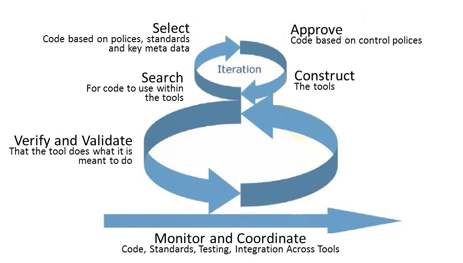
\includegraphics[width=5in]{Plan}
	\caption{High-Level Architecture}
	\label{fig-plan}
\end{figure}

Once at steady-state, each project will use 3-week (4 per quarter) sprints to develop and enhance their components. 
At the end of each sprint, integration across the feature sets will ensure coordination and compatibility.  
Experienced SLR authors and existing tool developers will have access to resulting sprint builds and have input into the product backlogs and priority assignments of these items (see attached support letters).  
Each team will construct a backlog of features that need to be developed for their specific feature set.
With the aid of the users of the specific features providing input, the project lead for each team will act as product owners to prioritize the backlog for each sprint.  
The graduate student will be responsible for high-level architecture and design decisions, including investigating various trade-offs in implementation choices.
The CAPS developers will implement and test the features in each sprint.
During the execution of the sprints and during the retrospectives at the end of the sprints we will identify cross-feature relationships and add them to the backlog for the appropriate feature sets.
The user communities for each of the feature sets will have the capability to be active testers to ensure features perform as expected.  

%The assignment of the feature sets will be based on needed expertise, current capabilities and programmatic learning objectives.  
%As an example of the programmatic learning objectives, CS students will be assigned to take the lead for core backplane tier features, while MIS students will take the lead for planning, coordination and monitoring features.  
%This assignment will draw on their experiences, coursework and career objectives.   
%Collectively the CS and MIS students will learn to work together and extend their professional comfort drawing upon the strengths of one another. 

\section{Project Schedule}
\label{sec:sched}
The schedule in Table~\ref{table-schedule} provides an overview of the number of development sprints planned for each quarter.  
It also provide an overview of other major activities planned each quarter such as Program Coordination and reviews by external (i.e., Non-UA) SLR  tool developers.  
Other reviews will be conducted at least every 9 months by external SLR authors and practitioners. 
The workshops for External Tool Developers and SLR Authors are also shown.   
The last item on the schedule shows the efforts that will take place to ensure the infrastructure is sustainable beyond the life of this grant. 

The project schedule considers multiple constraints and goals, for example:
\vspace{-8pt}
\begin{itemize}
	\item SAInT Feature Integration will ramp up during the first quarter (conducting 3 sprints) and then reach a steady state of 4 sprints for each of the next four quarters.  
	At the mid-point of the grant period, we will conduct a workshop with non-UA tool builders and SLR authors.  
	\item Preparing for the workshop and responding to feedback will reduce the number of sprints in the Winter 2017-18 quarter (after which 4 sprints per quarter will resume).  
	\item In the last 3 quarters of the project, the number of sprints will be ramped down as more user testing and training activities ramp up.
	\vspace{-4pt}
\end{itemize}
\vspace{-4pt}

\begin{table}
	\centering
	\caption{Project Schedule}
	\label{table-schedule}
	\begin{table}[!bth]
\caption{Project Schedule}
\label{tab:Schedule}
{\footnotesize 
\begin{tabular}{p{.48\textwidth}|c@{~}c@{~}c@{~}c|c@{~}c@{~}c@{~}c|c@{~}c@{~}c@{~}c|}
\cline{2-13}
	&   \multicolumn{12}{c|}{\textbf{Quarters}}  \\
	&   \multicolumn{4}{c}{Year 1}      & \multicolumn{4}{c}{Year 2}     & \multicolumn{4}{c|}{Year 3}      \\
	Tasks                          & Fall & Wint & Spr & Sum & Fall & Wint & Spr & Sum & Fall & Wint & Spr & Sum \\
\hline
	Program Coordination           & x    & x    & x   & x   & x    & x    & x   & x   & x    & x    & x   & x   \\
\hline
	\textbf{Initialize} - Analyze \& choose AI/Text-mining tools \& Identify data outputs for SLR phases       & x    & x    & x   & x   &     &     &    &    &     &     &    &    \\
\hline
	\textbf{Compose} - AI/Text-mining tools \& Data model for SLR phases       & x    & x    & x   & x   & x    &  x   & x   & x   & x    &  x   &x    & x  \\
\hline
	\textbf{Popularize} - Conduct one-on-one case studies  &     &     &    & x   &     &  x   &    & x   &     & x    &    & x   \\
\hline
	\textbf{Popularize} - Workshops                     &      &      &      &  x   &      &     &     &     &      &      &     &   x  \\
\hline
	\textbf{Support} - Use Helpdesk &      &      &      &     & x     & x    &x     & x    & x     & x     & x    & x    \\
\hline
	\textbf{Audit} - Tune AI/Text-mining approaches \& Conduct human-based studies                     &  x    &   x   &   x  &  x   &    x  &   x  &  x  &   x  &   x   &  x   &   x  & x   \\\cline{2-13}

\end{tabular}
}
\end{table}
\end{table}


\part{Results of Prior NSF Support}
% $Id: part_prior.tex 3082 2012-10-23 19:38:07Z jcarver $

NSF CCF-0915559 (PI: Kraft, Co-PI: Carver), (2009-present), Title: \emph{SHF: Small: Collaborative Research: Improved Code Clone Categorization}. In this project, PIs Kraft and Carver are developing and evaluating methods for categorizing code clone information to make it useful for developers. This project has supported the work of six graduate students. To date, this project has led to six workshop/conference~\cite{Beard_et_al:11,Carver_et_al:11,Chatterji_et_al:11,Chatterji_et_al:10,Chatterji_et_al:12,Corley-etal:12} papers and three journal publications~\cite{Lukins_et_al:10,JeremyRPate_et_al_2011,Biggers-etal:12}.

Co-PI Hale has no results in the previous 5 years.

% vim:syntax=tex


% vim:syntax=tex
